\section{Modelling articulated subjects}

% Brief introduction and discuss 'non-shape/weak shape' methods. E.g. faces and hands.
% Discuss methods like dolphins or Angjoo birds which start

% face model paper: https://arxiv.org/pdf/1909.01815.pdf

The design of 3D morphable models (3DMMs) has a significant recent history in computer vision research. A 3DMM is a statistical model designed to represent the structure, deformation and apperance space of for a particular object category. Such a model can be constructed for any object category for which a dense point-to-point correspondence can be established between instances. For example, a 3DMM can be designed to represent medium-sized quadrupeds but perhaps not for general animal categories. How, for instance, would one sensibly determine correspondences between a dog and an octupus? 3DMMs have been used extensively as a strong 3D prior to aid various 3D reconstruction algorithms. They are, however, most influential for problems with the most ambiguity: particularly when dealing with articulated objects (e.g. animals or humans), when only a single monocular RGB image is available or when no paired 3D training data is available. 

% cars: 
% ears: https://core.ac.uk/download/pdf/158370989.pdf
% human bodies: http://grail.cs.washington.edu/projects/digital-human/pub/allen03space-submit.pdf
% human bodies: 

Blanz and Vetter~\cite{blanz-vetter} presented the first 3DMM, which expressed a low-dimensional face space space learnt by aligning various face scans. This work, presented over two decades ago, has been recognized with an impact paper award for the continued applications for the ideas presented. Indeed, the approach introduced has found applications far beyond faces~\cite{face-warehouse, basel-old, basel-new}, including for cars~\cite{deformable-cars}, other human body parts including the hands~\cite{Khamis_2015_CVPR} and ears~\cite{deformable-ears}, the human body surface~\cite{anguelov05scape,loper15smpl} and a restricted set of animal categories~\cite{cafm, zuffi2017menagerie}.


This section will cover methods for modelling articulated subjects, focussing primarily methods for human bodies and animals. 


% \subsection{Building 3D morphable models}

%     Of primary concern to this thesis are methods which represent articulated structures, such as human bodies or animals, with a 3D polygon mesh. A polygon mesh $M = (V, T)$ is a collection of vertices, edges bound by vertex pairs, and polygons bound by sequences of edges and vertices~\cite{smith2006vertex}. Although other convex shapes are allowed, this thesis only has need to discuss triangular mesh polygons, which henceforth will be referred to as \emph{triangles}. An example mesh is shown in Figure~\ref{fig:polygon_mesh}. 
            
%         \begin{figure}[H] % Example image
%             \center{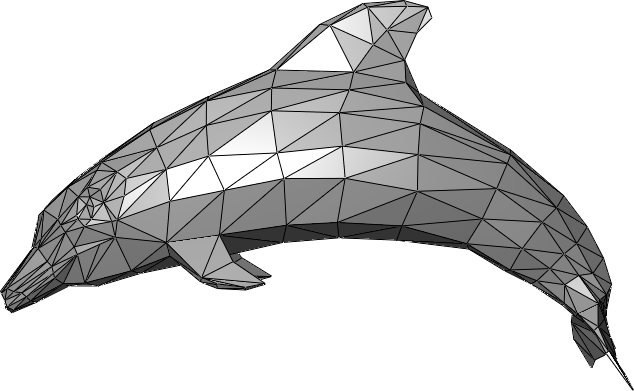
\includegraphics[width=0.5\linewidth]{dolphin_mesh}}
%             \caption{A polygon mesh~\cite{polygon_mesh}.}
%             \label{fig:polygon_mesh}
%         \end{figure}
    
 
%     \subsection{Mesh deformation}
%     The process of adapting a 3D mesh is known as \textit{mesh deformation} and has relevance to a multitude of computer graphics applications, particuarly those in which models are designed to represent dynamic objects. To constrain an optimization function (or simplify the animation process), it is useful to introduce priors that prevent unnatural mesh movement. Two methods for achieving this are discussed:


%         \subsubsection{As Rigid as Possible}
%         As Rigid as Possible (ARAP) surface deformation~\cite{sorkine2007rigid} is a distance function that measures similarity between two meshes with corresponding vertices. For two vertex sets~$V_{1}$ and~$V_{2}$, ARAP minimizes over~$N = |V|$ rotation matrices. Note~$j \sim i$ indicates vertex indices~$j$ adjacent to vertex index~$i$:

%         \begin{equation}
%             D(V_{1}, V_{2}) = \min_{R_{1..N}}\sum_{i=1}^{N}\sum_{j \sim i}|| (V_{1i} - V_{1j}) - R_{i}(V_{2i} - V_{2j}) ||^{2}
%         \end{equation}

%         This distance function can be incorporated into an energy-based optimizer as a regularization function. By considering how small vertex regions overlap, the function can be used to  discourage `unnatural movement', e.g.\ shearing effects, over mesh faces. ARAP regularizers are particularly useful in cases in which there is no prior knowledge of the mesh. Figure~\ref{fig:arap_dino} shows an example of a dinosaur mesh undergoing ARAP deformation, obtained by translating the highlighted yellow vertex.

%         \begin{figure}[H] % Example image
%             \center{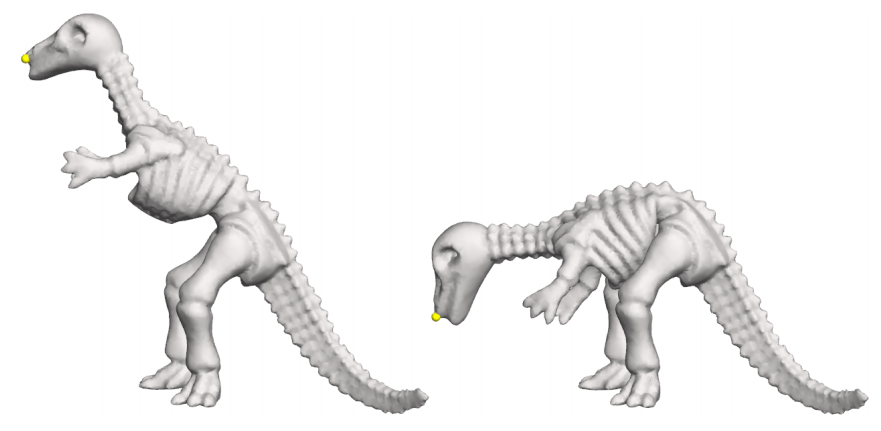
\includegraphics[width=0.35\linewidth]{dino_arap}}
%             \caption{Dinosaur mesh undergoing ARAP deformation, obtained by translating the highlighted yellow vertex. Reprinted from~\cite{sorkine2007rigid}.}
%             \label{fig:arap_dino}
%         \end{figure}


%         \subsubsection{Skeletal Rigging and Linear Blend Skinning}
%         In cases that the mesh shape is known in advance, it is common to follow a process known as \textit{rigging}, in which the mesh is augmented with a hierarchical bone structure. The point at which two bones meet is called a \emph{joint}, and these can be used to define acceptable centres of rotation for mesh deformation. It is possible to describe a distribution of joint configurations, which could be used to constrain the mesh to (in the case of human / animal subjects) anatomically achievable poses. It is also simple to define conceptual `body parts' from a rigged mesh, by considering regions between pairs of joints; for example a lower leg region can be defined between a knee and ankle joint. A simple example of a rigged 2D mesh with joints indicated by green diamonds is shown in Figure~\ref{fig:finger_model}. Note how the mesh surface deforms naturally as the joints are displaced.
        
%         \begin{figure}[H]
%             \centering
%             \begin{subfigure}{0.48\linewidth}
%             \centering
%                 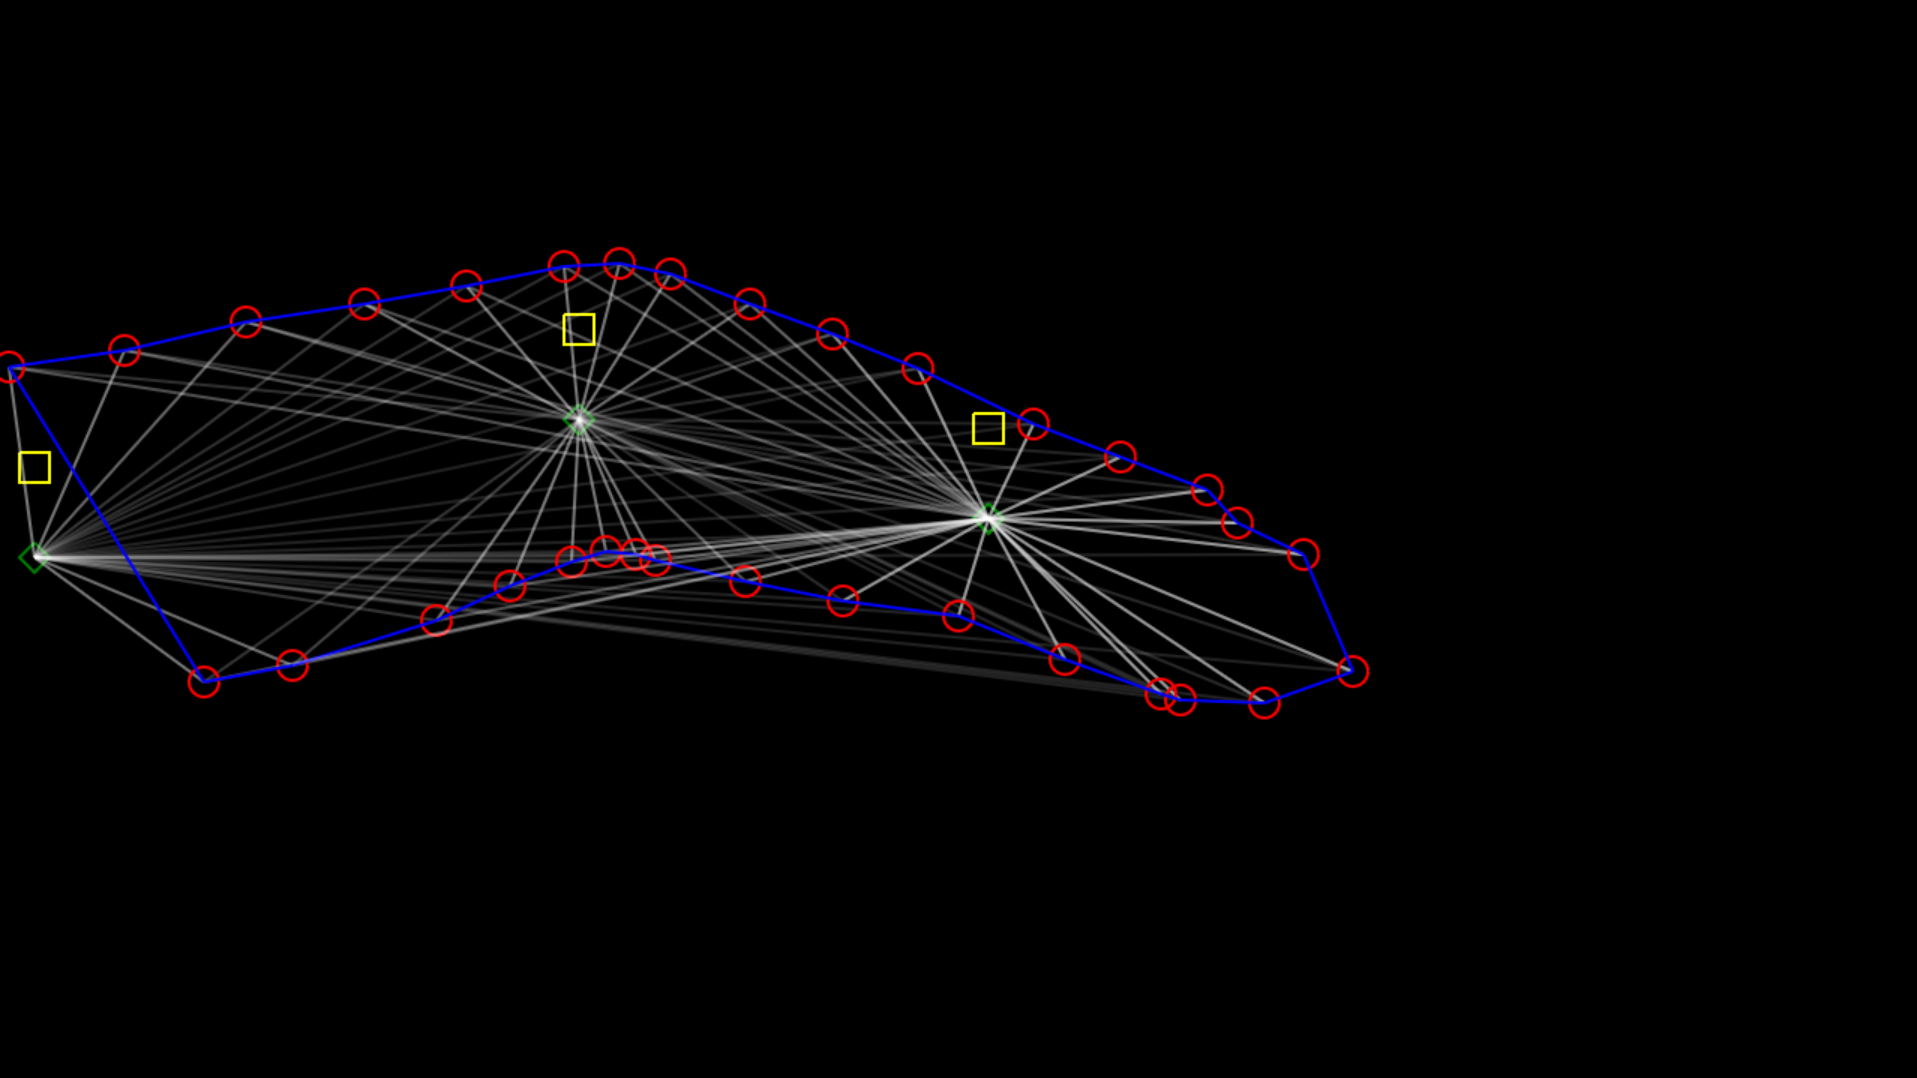
\includegraphics[width=1\linewidth]{finger/finger1}
%                 \caption{Default joint positions.}
%             \end{subfigure}
%             \begin{subfigure}{0.48\linewidth}
%             \centering
%                 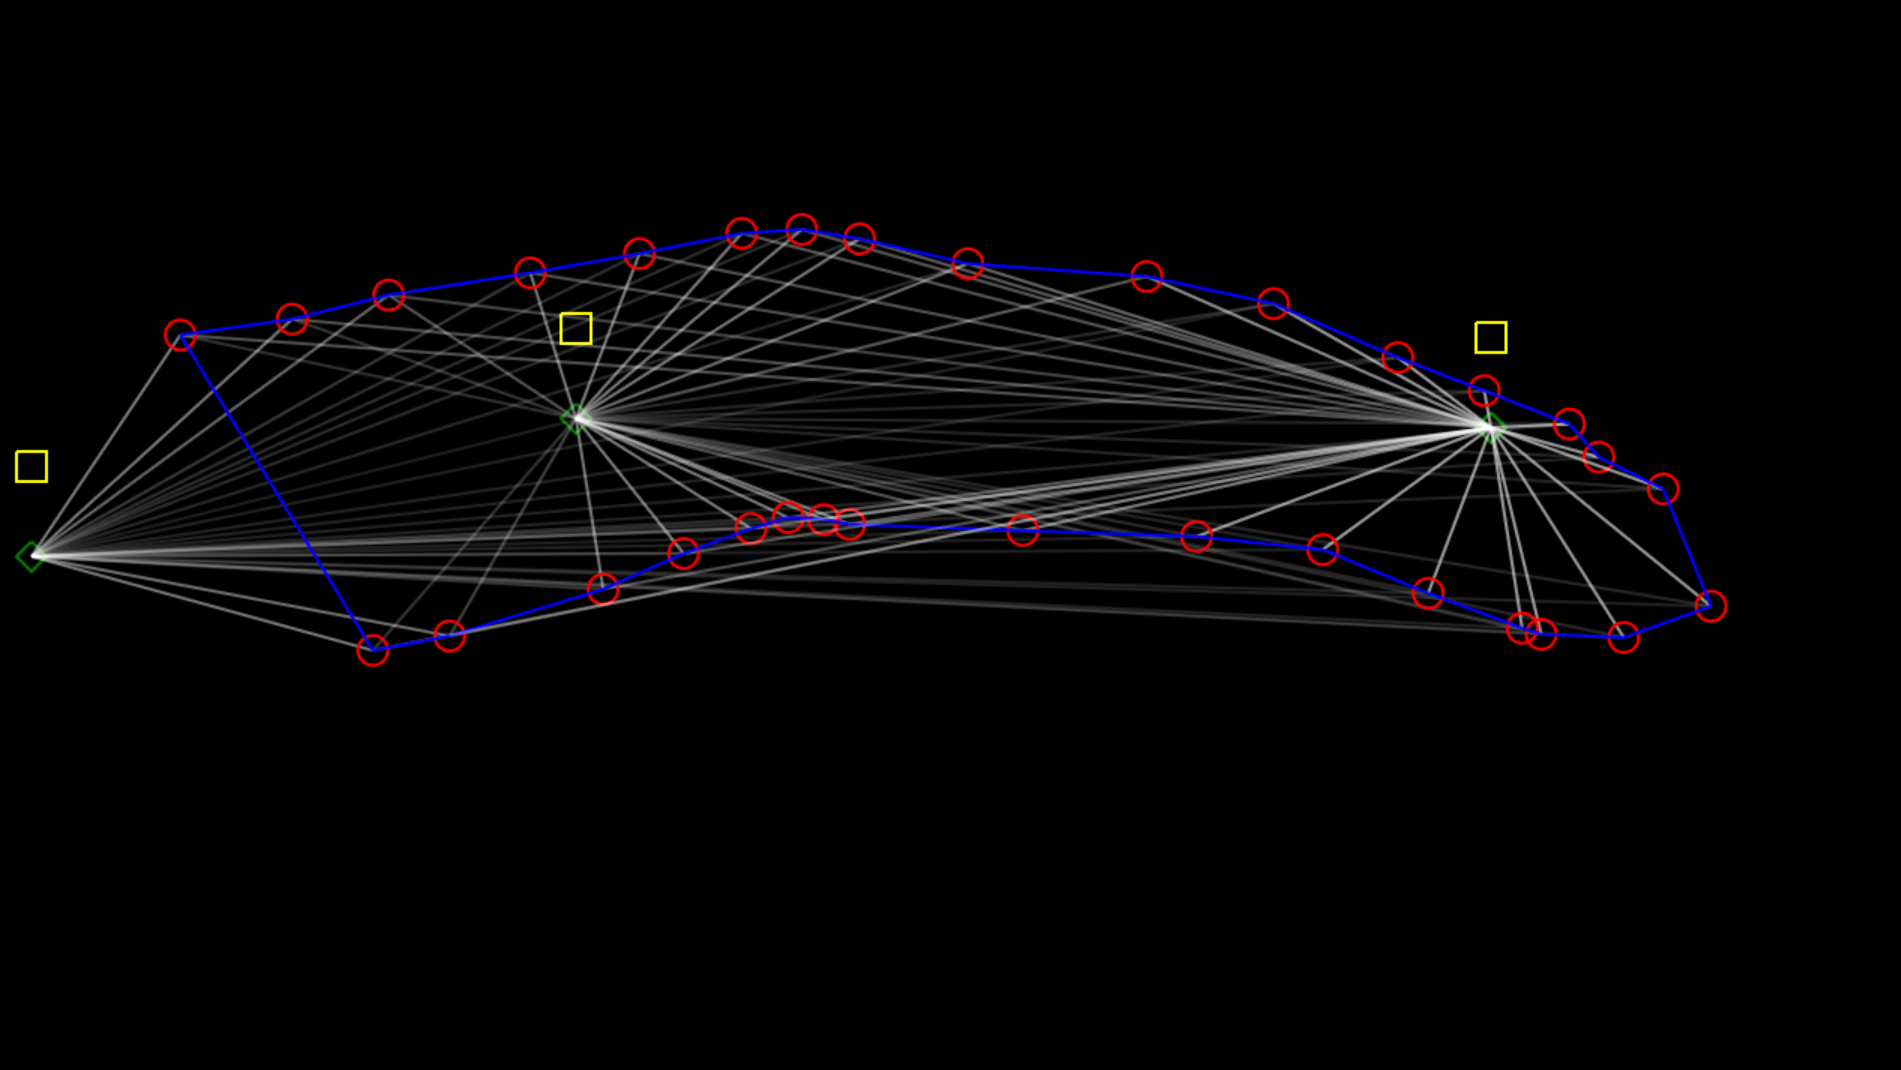
\includegraphics[width=1\linewidth]{finger/finger2}
%                 \caption{Right-most joint displaced.}
%             \end{subfigure}
%             \begin{subfigure}{0.48\linewidth}
%             \centering
%                 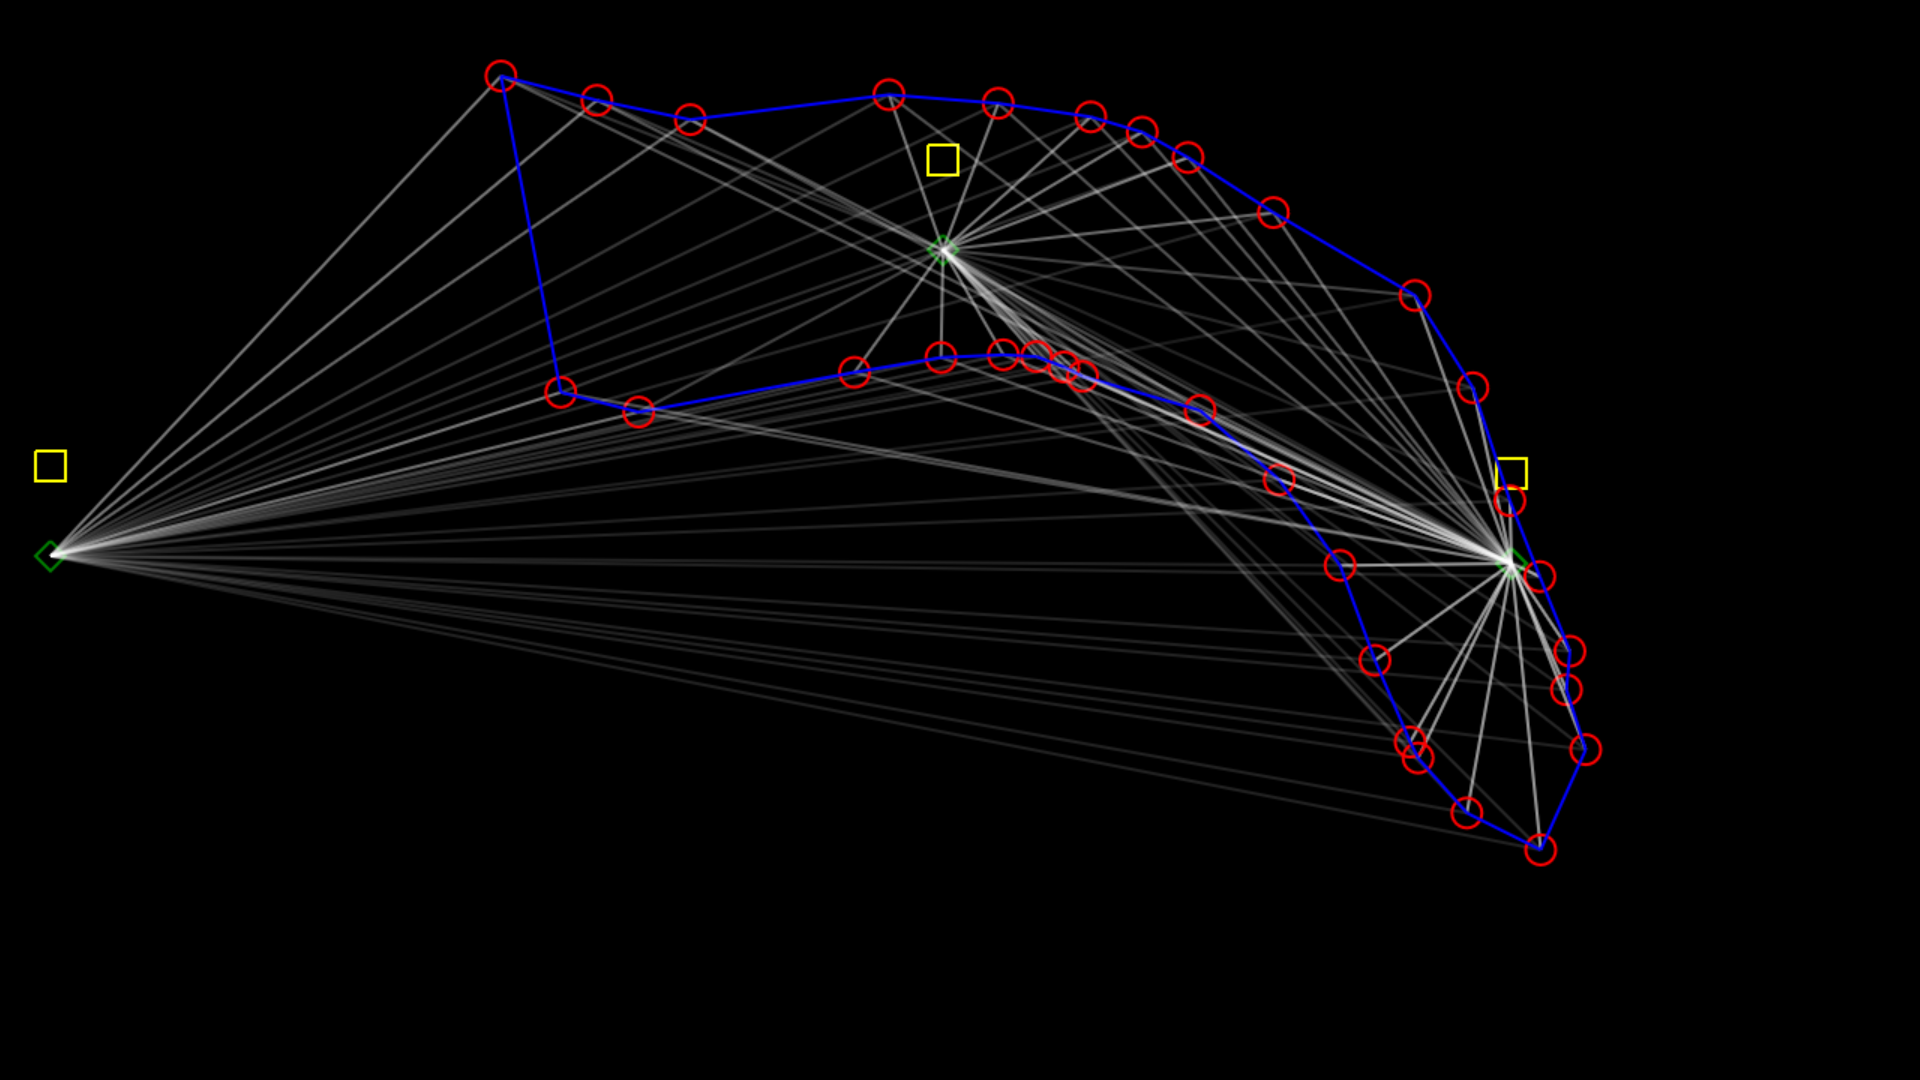
\includegraphics[width=1\linewidth]{finger/finger3}
%                 \caption{Central joint displaced and right-most joint displaced and rotated.}
%             \end{subfigure}%
%             \caption{Web application demonstrating LBS on a 2D finger mesh. Joints are denoted as green diamonds.}
%             \label{fig:finger_model}
%         \end{figure}

%         \clearpage
%         Formally, a skinned mesh consists of a set of rigged vertices $V \subseteq \mathbb{R}^3 \times \mathbb{R}^{|J|}$, a set of faces $F \subseteq V^3$ and joints $J \subseteq R^{3\times3}$. Each vertex $v = (x, s) \in V$ consists of positional coordinate $x \in \mathbb{R}^{3}$ and a weight vector $s \in \mathbb{R}^{|J|}$ which describes the level of influence each joint $j \in J$ has over its movement. Many approaches exist for assigning weights, but perhaps the simplest is to build a vector with entries corresponding to the distance from the vertex to each joint centre. Skinning weight vectors are normalized such that their entries sum to one, and for computational reasons, the number of non-zero elements is typically limited to 2 or 4. The weakness of such models is that artifacts and other unrealistic deformations can occur around the model joints, particularly for meshes that model non-linear structures such as humans. However, the technique is frequently used in computer graphics and game design when a character's shape is known ahead of time.

%         To assist in explanation, Figure \ref{fig:rigged_cylinder} shows skinning weight influences from three joints within a rigged cylinder mesh. Here, $|J| = 3$ and each vertex $v_{i} = (x_{i}, s_{i}) \in V$ has a skinning weight vector $s_{i} \in \mathbb{R}^{3}$. Each model joint is assigned a distinct RGB value, shown separately in (a), (b) and (c), and together in (d) by linearly combining the colours. This linear blend colorization scheme will be frequently used in later sections of this report.

%         \begin{figure}[H]
%             \centering
%             \begin{subfigure}{0.25\linewidth}
%             \centering
%                 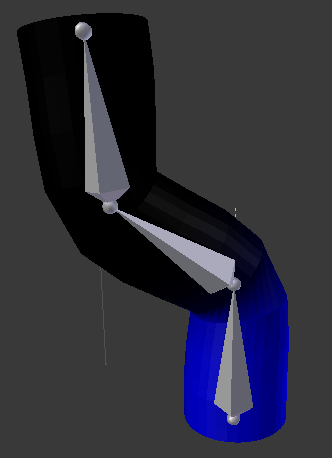
\includegraphics[width=1\linewidth]{wonky_pole/lower_bone}
%                 \caption{Lower joint.}
%             \end{subfigure}%
%             \begin{subfigure}{0.25\linewidth}
%             \centering
%                 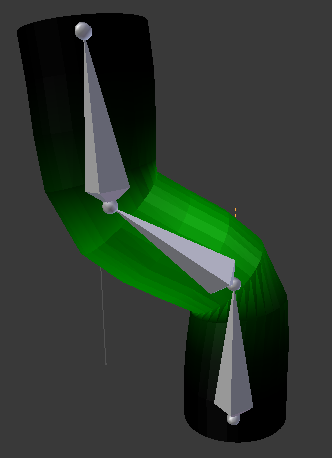
\includegraphics[width=1\linewidth]{wonky_pole/middle_bone}
%                 \caption{Middle joint.}
%             \end{subfigure}%
%             \begin{subfigure}{0.25\linewidth}
%             \centering
%                 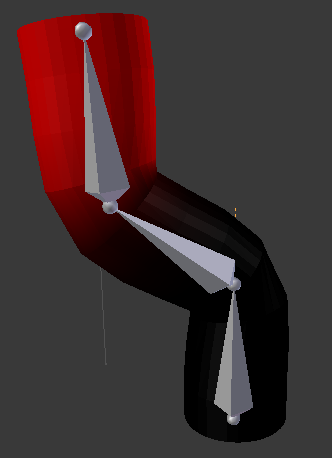
\includegraphics[width=1\linewidth]{wonky_pole/upper_bone}
%                 \caption{Upper joint.}
%             \end{subfigure}%
%             \begin{subfigure}{0.25\linewidth}
%             \centering
%                 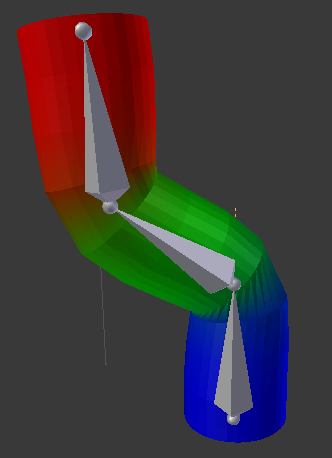
\includegraphics[width=1\linewidth]{wonky_pole/linear_blend}
%                 \caption{Linear blend.}
%             \end{subfigure}%
%             \caption{A rigged cylinder with $|J| = 3$ and where each vertex $v_{i} = (x_{i}, s_{i}) \in V$ has a skinning weight vector $s_{i} \in \mathbb{R}^{3}$.}
%             \label{fig:rigged_cylinder}
%         \end{figure}

%         Figure \ref{fig:rigged_quadruped} shows a more complex rigged quadruped mesh with $|J| = 25$ with skinning weight influences again shown by the linear blend colorization scheme. Again, each joint is assigned a unique RGB value and a vertex's colour is calculated by linearly combining joint colours with skinning weight vectors given by the $\{s_{i}\}$. A triangle's colour is then generated by averaging the colours given for the three surrounding vertices.

%         \begin{figure}[H] % Example image
%             \center{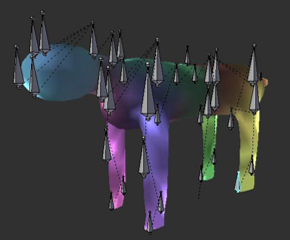
\includegraphics[width=0.5\linewidth]{linear_blend_bold_bones}}
%             \caption{A rigged quadruped with $|J| = 25$ and where each vertex $v_{i} = (x_{i}, s_{i}) \in V$ has a skinning weight vector $s_{i} \in \mathbb{R}^{3}$. Visualization uses the linear blend colorization scheme in which each joint is assigned a unique RGB value.}
%             \label{fig:rigged_quadruped}
%         \end{figure}

%         Once a mesh has been suitably rigged, there are a number of options (e.g. Linear Blend Skinning (LBS), Dual Quaternions~\cite{kavan2007skinning} etc.) for applying a particular mesh deformation. Typically, a user assigns a transformation (in this case comprising a rotation and transformation) to each `joint' and the updated positions $\bar{x_{i}}$ of the remaining vertices $v_{i}$ with original positions $x_{i}$ are then calculated. The original transformation for each joint (i.e. before the deformation) is expressed as a matrix $U_{j}$. The transformation after the deformation has been applied is captured by $D_{j}$. Note that $s_{ij}$ denotes the skinning weight influence of joint~$j \in J$ on vertex $v_{i} \in V$.
        
%         The updated positions $\bar{x_{i}}$ can then be calculated by LBS:

%         \begin{equation}
%             \bar{x_{i}} = \sum_{j=1}^{|J|}s_{ij}D_{j}U_{j}^{-1}x_{i}
%         \end{equation}


% \subsection{Modelling human body parts}

% % Hands, faces etc.


% Given the availability of strong shape and pose priors, articulated hand tracking aptly demonstrates the advantage of model fitting approaches. Again, it is first necessary to decide how the human hand should be parameterized, i.e. what an optimizer should specifically aim to learn. Similar to the case with the full human body, the aim is again to adapt a mesh (although this time of a hand) to reproduce a performance given by a real human hand either in still frames or from an input video sequence. Many modern approaches follow a hand parameterization given by Khamis et al.~\cite{Khamis_2015_CVPR} using a pose vector $\theta \in \mathbb{R}^{28}$ that includes global translation and rotation, one adbuction and three flexion variables for each finger digit, and one abduction and flexion parameter for the wrist and forearm. An example hand tracking result can be seen in Figure~\ref{fig:hand_tracking}. 

\subsection{Constructing 3D morphable models}


% As it relates to modelling rigged articulated objects, it is important to factor deformation into two categories. Firstly \emph{pose} deformations govern the positioning of articulated parts, for example arms and legs. Consequently, parameters for controlling pose will typically vary when reconstructing a sequence exhibiting an articulated subject in motion. \emph{Shape} deformations, however, control the relative lengths and sizes of articulated parts and indeed the global structure. In general, parameters for controlling shape should be invariant to motion and remain consistent for a single individual. 
      
% A frustrating exception to this occurs in the literature discussing face reconstruction. Since models typicaly  since without a define face skeleton, all shape variations are handling face reconstruction, since without a defined face skeleton, all 

% remain consistent In general,  control the relative length and sizing of body parts. In general, only one sizing and length of the model limbs (e.g. arms and legs). typically used to govern the positions of the limbs. are used to govern global and local body proportions (e.g. body part sizes and lengths), and are mostly consistent for a single subject. \emph{Pose deformations} on the other hand are used to govern the positioning of limbs. In order to consolidate various definitions used in the literature, this thesis will define \emph{pose} to be any mesh deformation affected by the movement of an internal skeleton. \emph{Shape} will therefore be any other kind deformation. As an example, then, of most concern to 3D morphable models representing human faces will be \emph{shape} parameters, since face models rarely have an internal skeletal structure. an internal skeleton constitute any deformation change affected by the typically which govern body proportions (e.g. body part sizes, lengths) and \emph{pose deformation} which governs the positioning of limbs. Of course, a typical image of a human or animal will comprise 

3D deformable models are typically represented by a polygon mesh. A polygon mesh $M = (V, T)$ is a collection of vertices, edges bound by vertex pairs, and polygons bound by sequences of edges and vertices~\cite{smith2006vertex}. Although other convex shapes are allowed, this thesis only has need to discuss triangular mesh polygons, which henceforth will be referred to as \emph{triangles}. An example mesh is shown in Figure~\ref{fig:polygon_mesh}. 

\begin{figure}[H] % Example image
    \center{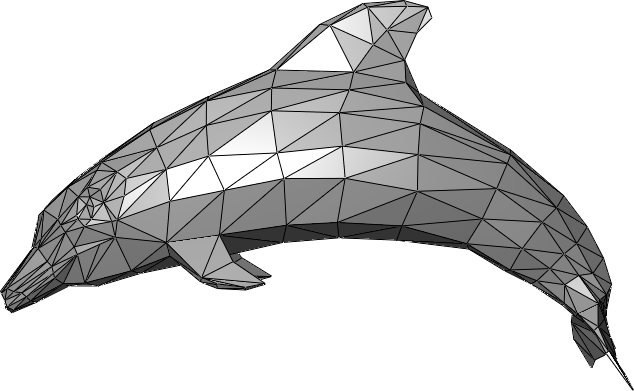
\includegraphics[width=0.5\linewidth]{dolphin_mesh}}
    \caption{A polygon mesh~\cite{polygon_mesh}.}
    \label{fig:polygon_mesh}
\end{figure}

A 3D morphable model can then be constructed by deforming a template mesh $M$ on $n$-vertices to a set of 3D training examples. Generally, this optimization will have a significant degrees of freedom so it is necesssary to employ techniques for regularization. One such regularizer is known as the \emph{As Rigid as Possible} scheme: 

\begin{definition}[As Rigid as Possible]
As Rigid as Possible (ARAP) surface deformation~\cite{sorkine2007rigid} is a distance function that measures similarity between two meshes with corresponding vertices. For two vertex sets~$V$ and~$W$, ARAP minimizes over~$N = |V|$ rotation matrices. Note~$j \sim i$ indicates vertex indices~$j$ adjacent to vertex index~$i$:

\begin{equation}
    D(V, W) = \min_{R_{1..N}}\sum_{i=1}^{N}\sum_{j \sim i}|| (V_{i} - V_{j}) - R_{i}(W_{i} - W_{j}) ||^{2}
\end{equation}

This distance function can be incorporated into an energy-based optimizer as a regularization function. By considering how small vertex regions overlap, the function can be used to  discourage `unnatural movement', e.g.\ shearing effects, over mesh faces. ARAP regularizers are particularly useful in cases in which there is no prior knowledge of the mesh. Figure~\ref{fig:arap_dino} shows an example of a dinosaur mesh undergoing ARAP deformation, obtained by translating the highlighted yellow vertex.

\begin{figure}[H] % Example image
    \center{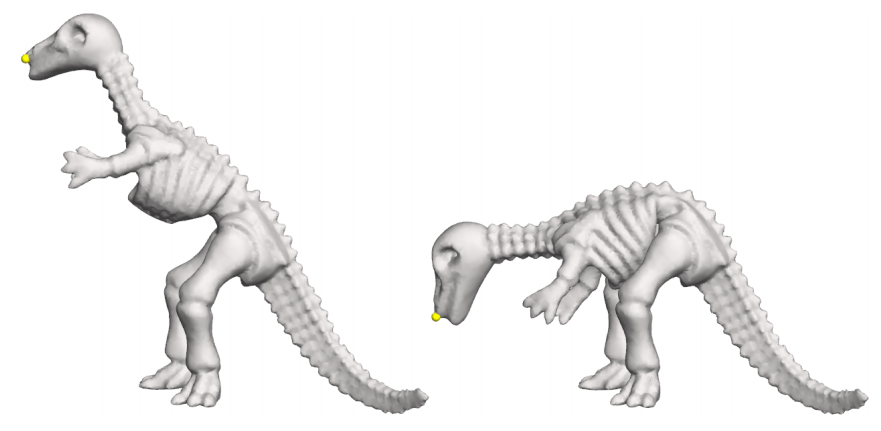
\includegraphics[width=0.35\linewidth]{dino_arap}}
    \caption{Dinosaur mesh undergoing ARAP deformation, obtained by translating the highlighted yellow vertex. Reprinted from~\cite{sorkine2007rigid}.}
    \label{fig:arap_dino}
\end{figure}      

\end{definition}

Once aligned, a $d$-dimensional \emph{shape space} can then be defined (with $d << n$), where each $w \in \R{d}$ gives rise to a vertex configuration in $\R{3}$ (with unchanged triangulation). In this way, every plausible 3D example has a parameter vector $w \in \R{d}$ that generates it. This construction can then be interpreted as a \emph{generative} model. However, very few selections of $w \in \R{d}$ will generate a plausible-looking 3D mesh. This can then be interpreted probabilistically, by defining a density function $f(w)$ that defines the likelihood that a realistic 3D example would be represented by $w$ in shape space. 

\subsection{Modelling shapes (e.g. faces)}

The concepts raised above were first introduced in the seminal work of Blanz and Vetter~\cite{blanz-vetter}. They define a linear generator function based on principle component analysis (PCA) in order to map $d$-dimensional parameter vectors to the set of $n$ vertex coordinates. In particular they use the mapping:

\begin{equation}
    g(\alpha) = \bar{c} + E\alpha
\end{equation}

where $g: \R{d} \mapsto \R{3n}$ is the generator function, $\bar{c} \in \R{3n}$ is the mean 3D face in the training dataset and $E \in \R{3n \times d}$ is a matrix containing the $d$ most dominant eigenvectors computed over shape residuals $\{c_i - \bar{c_i}\}$. 

This construction assumes 3D faces in this $d$-dimensional parameter space follow a multivariate normal distribution (a concept explored further in this thesis Chapter 4). In addition, the function $f(w)$ which defines the likelihood shape space vector $\alpha$ represents a plausible face, is therefore given by the Mahalanbois distance of $\alpha$ to the origin. 

Note that this formulation additionally enables the definition of facial expressions. For example, Blanz and Vetter defined an expression (e.g. surprise) according to the difference in shape space between a expressive and neural face of the same subject. This then enabled the formulation above to be factored into identity and expression components:

\begin{equation}
    g(\alpha_{idt}, \alpha_{exp}) = \bar{c} + E_{idt}\alpha_{idt} + E_{exp}\alpha_{exp}
\end{equation}

where $E_{idt}, E_{exp}$ are the basis vectors of the identity and expression space and $\alpha_{idt}, \alpha_{exp}$ are the coefficients. As noted by Lewis et al.~\cite{xxx}, the basis vectors of the expression space above can be interpreted as a data-driven \emph{blendshape model}: a standard approach in the animation industry for representing facial expressions as a linear combination of target faces. This concept will later reemerge in a section discussing corrective blendshapes uses in SMPL~\cite{loper15smpl}.

%Blendshape Facial Animation
As identified by Blanz and Vetter, improved modelling of finer details (particularly around the eye or nose regions) can be obtained through local modelling. Various authors~\cite{xxx} began manually segmentating the face into parts and learning individual PCA representations for them. Later, segmentations were automatic and learned based on displacement patterns found in the training dataset. Next, approaches were adopted based on hierarchical, multi-scale frameworks~\cite{xxx, xxx}. Possibly the closest to later sections which require a focus on \emph{pose deformation}  is the work of Wu et al~\cite{xxx}. who combine a a local shape space model with an anatomical bone structure that helps regularize deformation. 

% booth et al 2017
% pascal 2010
% egger et al 2016b
% zhou et al.
% xu et al (deep 3d portrait from a single image)

A standard challenge in face modelling is towards reconstructing appearance, typically incorporating albedo and illumination (although frequently these are not factored, in which case apperance is generally referred to as \emph{texture}). Early work modelled shape and texture independently~\cite{xxx, xxx}, although recent techniques show solving for these factors jointly enable constraints to be applied due to correlations present. Perhaps most interesting are the recent techniques among these~\cite{xxx, xxx}, who propose methods based on deep convolutional models to jointly model shape and texture.  

% PROBLEMS
% the statistics of most models are limited to the face and do not include information on eyes, mouth interior or hair
% Second, the interpretability of the representations would benefit from being improved. PCA is the most commonly used method to perform statistics on 3D faces, and as it is an unsupervised method, the principal components do not coincide with attributes that humans would use to describe a face


\subsection{Modelling articulation (e.g. hands)}


% Perhaps the biggest difference with hand modelling are the complex modes of articulation among subjects. 


3D morphable models have also influenced work in 3D hand tracking and modelling. Human hands servce multiple purposes in everyday life, serving a mechanism to handle tools/objects, expressing emotion and aiding (or even as the primary tool for) communication. As a result, hands (and particularly fingers) exhibit complex articulation patterns which are best characterized as 3D \emph{rotations}. Compared to the previous section, in which face shape variation could be represented as as an abstract linear basis learnt from scans, an advantage to modelling hands is the modes of articulation can be defined in advance. 

In particular, human hand motion is controlled by a hierarchical bone structure referred to as a \emph{skeleton}. The point at which two bones meet is referred to as a \emph{joint} and can be used to define acceptable centers of articulation. The direction and magnitude of the articulation can then be neatly expressed as a 3D rotation.

This formulation helps provide insight into why the abstract linear basis (shape space) introduced in the previous section would be poor choice for modelling hands. Deformation is here characterized in terms of 3D rotations, and 3D rotations are non-linear with respect to the input angle. This is easily shown: 

\begin{definition}[3D Rotations]
    

The simplest kind of 3D rotation is an \emph{elementary rotation} and involves a rotation around a single axis of a coordinate system. For example, the following matrix represents a rotation by an angle $\gamma$ around the $x$ axis:

\begin{equation}
    R_{x}(\gamma) = \begin{bmatrix}
        1 & 0 & 0 \\
        0 & \cos(\gamma) & -\sin(\gamma) \\
        0 & \sin(\gamma) & \cos(\gamma)
    \end{bmatrix}
\end{equation}

One can then apply this matrix to an input point $p \in \R{3}$ to compute the new position $p'$ after rotating $\gamma$ around the $x$ axis:

\begin{equation}
    p' = R_{x}(\theta)p
\end{equation}

This formulation can then be extended to represent any 3D rotation as the composition of elementary rotations. For example, a 3D rotation can be decomposed into a $\gamma$ rotation around the $x$-axis (pitch), followed by a $\beta$ rotation around the $y$-axis (yaw) and finally by an $\alpha$ rotation around the $z$-axis (roll). 

\begin{equation}  
    R = R_{z}(\alpha) R_{y}(\beta) R_{x}(\gamma)
\end{equation}

One can see immediately that affecting a 3D rotation (i.e. computing the new position of the points) is a non-linear function of the input angle. It is necessary, therefore to describe an alternative technique for low-dimensional and efficient mesh deformation, which relies on \emph{rigging} and \emph{linear blend skinning}. 

\end{definition}

% Compared to facesCompared to faces, hands have a simpler space of shape variation (typically restricted to palm size, finger lengths etc.) but the modes of articulation are extremely complex. In the class of 3DMMs, hand models arguably have the strongest synergy to their biological counterparts; in many cases each of the 27 hand bones (occasionally except the capal bones which join the fingers to the wrists) are explicitly represented in the model skeleton.

\begin{definition}[Skeletal Rigging and Linear Blend Skinning (LBS)]
    
In cases that the articulated object is known in advance, it is common to augment a representative 3D mesh model with an internal skeleton that approximates the biological counterpart. This is achieved through a process known as \emph{rigging}.  

% In general, the mesh skeleton approximates the real, biometric skeleton by allowing the important modes of deformation but often is a rough approximation of the real, biometric skeleton be detailed enough to allow the primary modes of deformation, but often it is not necessary that the 3D mesh skeletthat the articulated object is known In cases that the mesh shape is known in advance, it is common to follow a process known as \textit{rigging}, in which the mesh is augmented with a hierarchical bone structure. The point at which two bones meet is called a \emph{joint}, and these can be used to define acceptable centres of rotation for mesh deformation. It is possible to describe a distribution of joint configurations, which could be used to constrain the mesh to (in the case of human / animal subjects) anatomically achievable poses. It is also simple to define conceptual `body parts' from a rigged mesh, by considering regions between pairs of joints; for example a lower leg region can be defined between a knee and ankle joint. A simple example of a rigged 2D mesh with joints indicated by green diamonds is shown in Figure~\ref{fig:finger_model}. Note how the mesh surface deforms naturally as the joints are displaced.

% \begin{figure}[H]
%     \centering
%     \begin{subfigure}{0.48\linewidth}
%     \centering
%         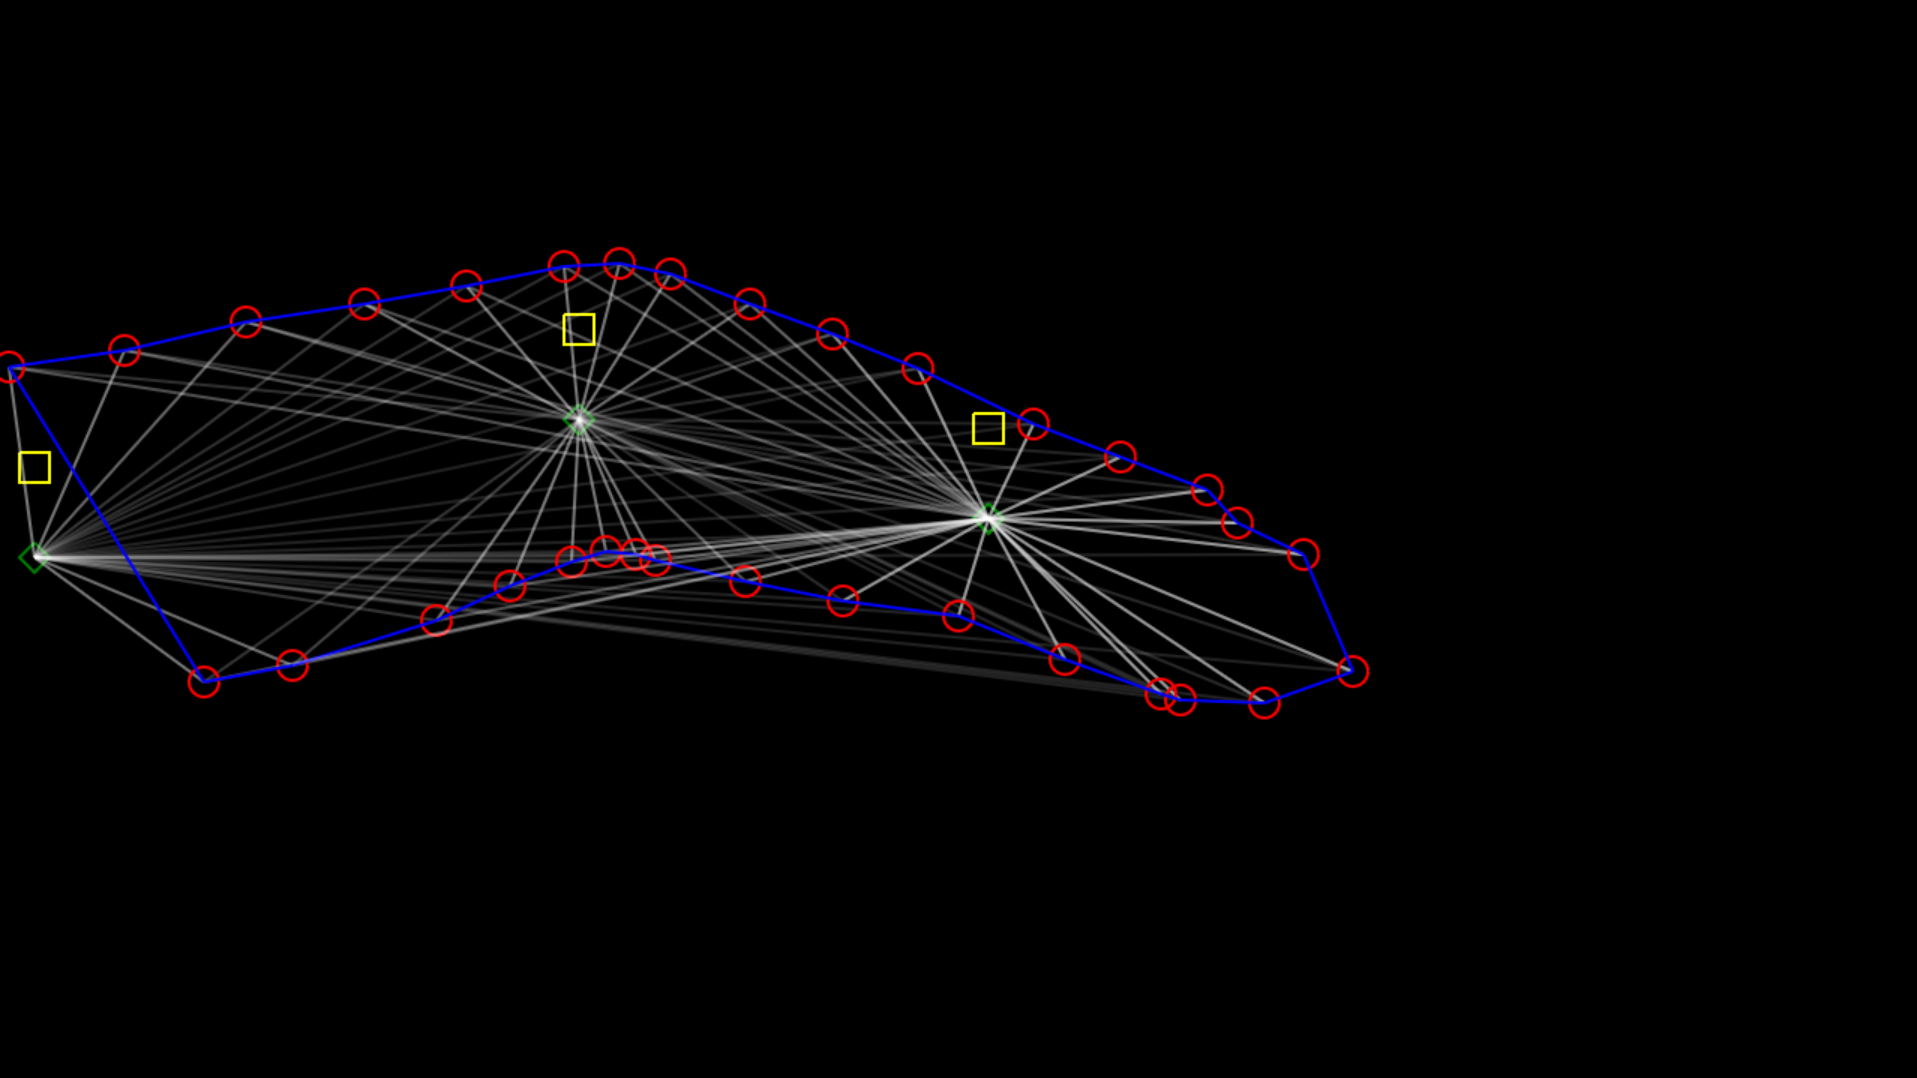
\includegraphics[width=1\linewidth]{finger/finger1}
%         \caption{Default joint positions.}
%     \end{subfigure}
%     \begin{subfigure}{0.48\linewidth}
%     \centering
%         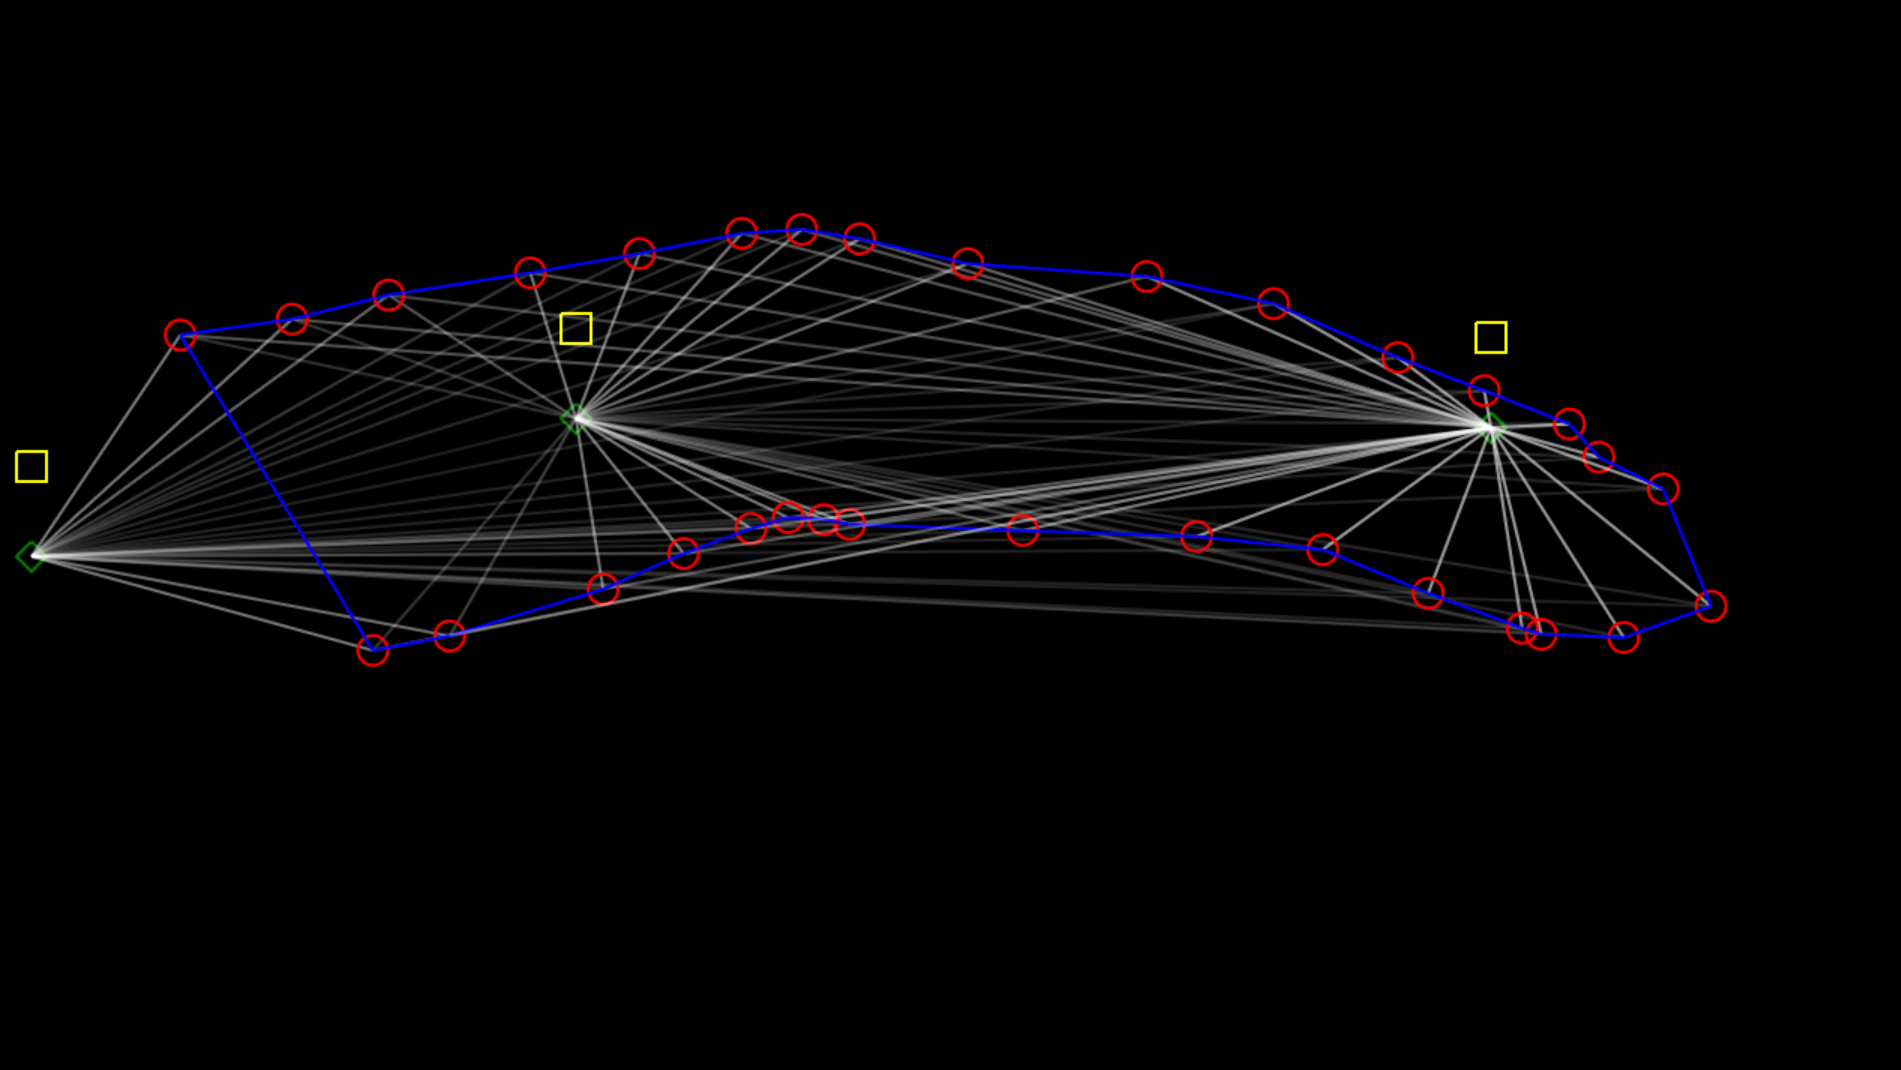
\includegraphics[width=1\linewidth]{finger/finger2}
%         \caption{Right-most joint displaced.}
%     \end{subfigure}
%     \begin{subfigure}{0.48\linewidth}
%     \centering
%         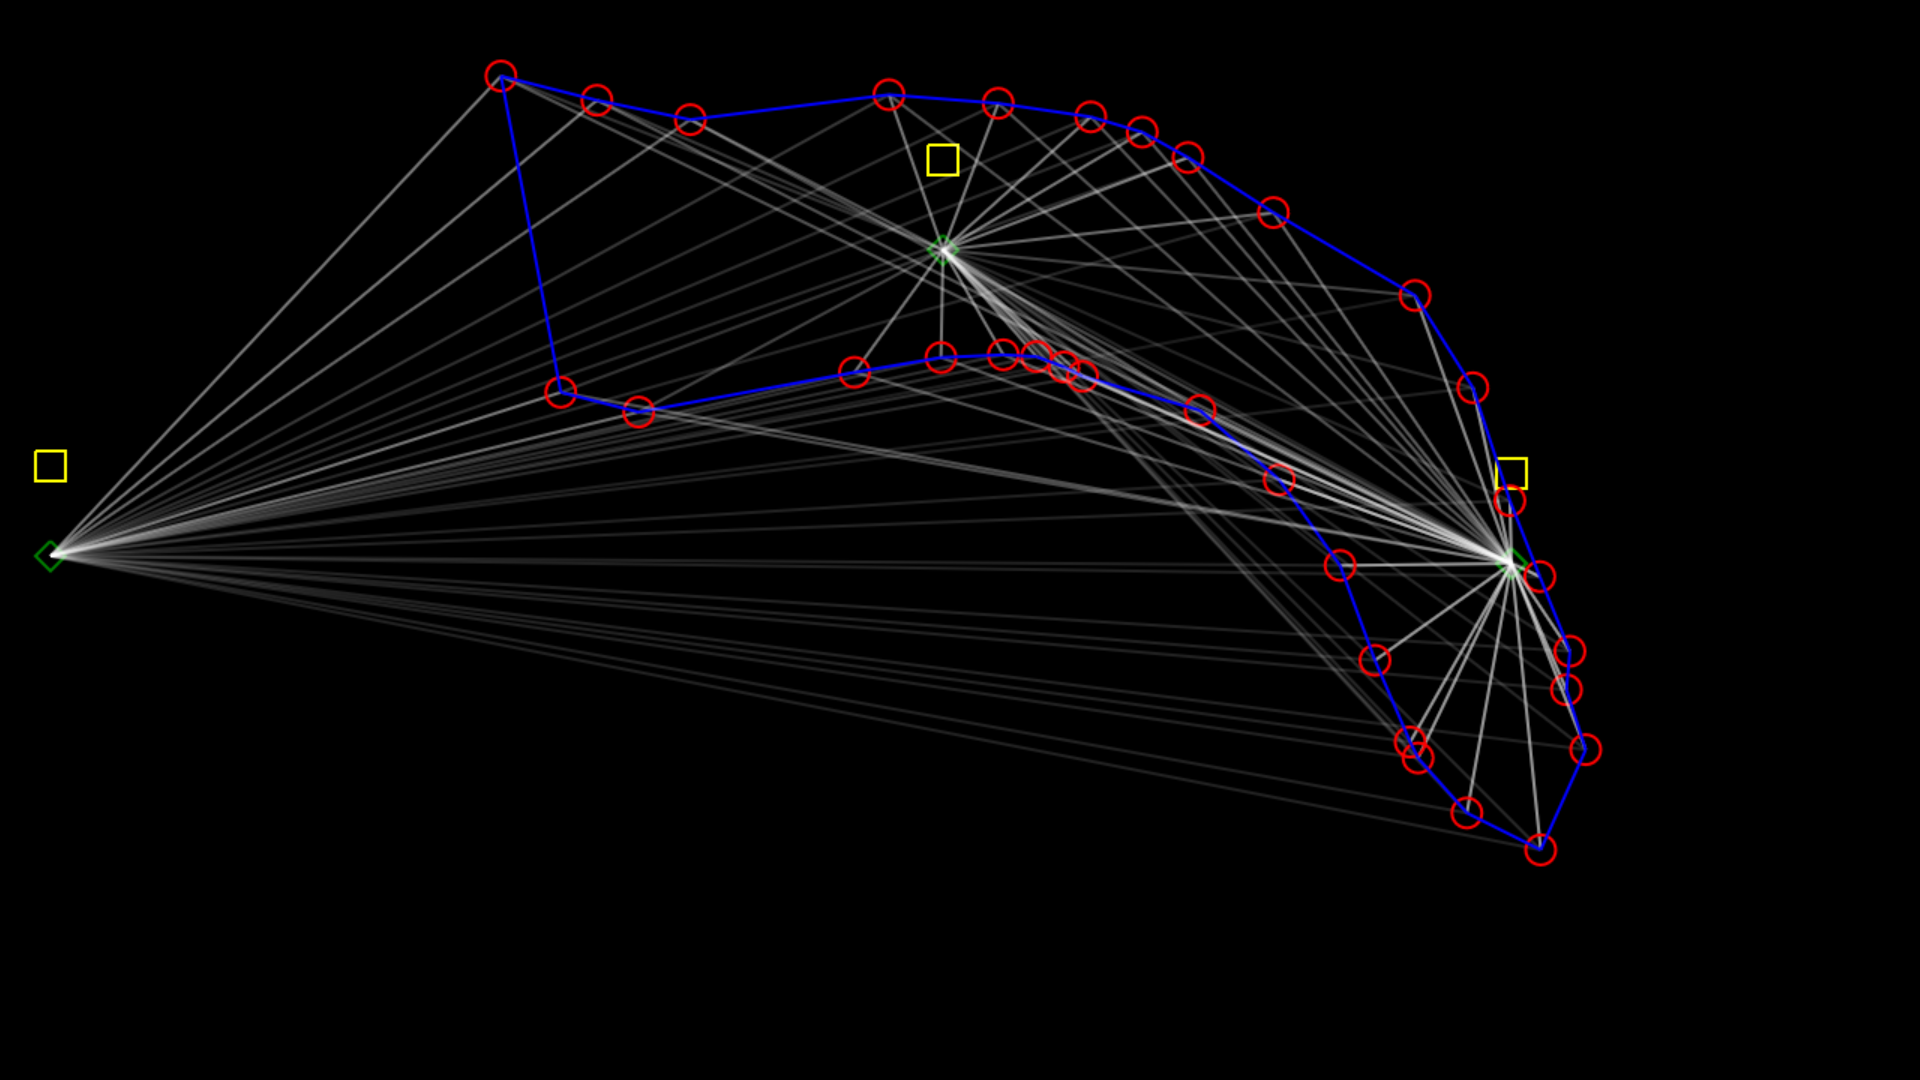
\includegraphics[width=1\linewidth]{finger/finger3}
%         \caption{Central joint displaced and right-most joint displaced and rotated.}
%     \end{subfigure}%
%     \caption{Web application demonstrating LBS on a 2D finger mesh. Joints are denoted as green diamonds.}
%     \label{fig:finger_model}
% \end{figure}

Formally, a skinned mesh consists of a set of rigged vertices $V \subseteq \R{3} \times \R{|J|}$, a set of faces $F \subseteq V^3$ and joint transformation matrices $J \subseteq \RR{3}{4}$. Each vertex $v = (x, s) \in V$ consists of positional coordinate $x \in \R{3}$ and a weight vector $s \in \R{|J|}$ which describes the level of influence each joint $j \in J$ has over its movement. Many approaches exist for assigning weights, but perhaps the simplest is to build a vector with entries corresponding to the distance from the vertex to each joint centre. Skinning weight vectors are normalized such that their entries sum to one, and for computational reasons, the number of non-zero elements is typically limited to 2 or 4. The weakness of such models is that artifacts and other unrealistic deformations can occur around the model joints, particularly for meshes that model non-linear structures such as humans. However, the technique is frequently used in computer graphics and game design when a character's shape is known ahead of time.

% To assist in explanation, Figure \ref{fig:rigged_cylinder} shows skinning weight influences from three joints within a rigged cylinder mesh. Here, $|J| = 3$ and each vertex $v_{i} = (x_{i}, s_{i}) \in V$ has a skinning weight vector $s_{i} \in \mathbb{R}^{3}$. Each model joint is assigned a distinct RGB value, shown separately in (a), (b) and (c), and together in (d) by linearly combining the colours. This linear blend colorization scheme will be frequently used in later sections of this report.

% \begin{figure}[H]
%     \centering
%     \begin{subfigure}{0.25\linewidth}
%     \centering
%         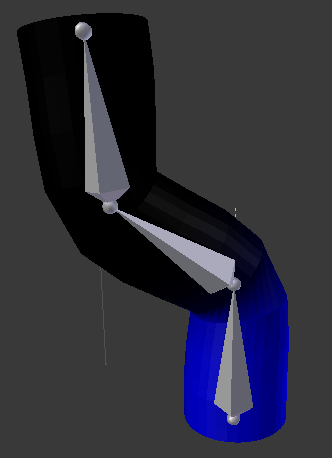
\includegraphics[width=1\linewidth]{wonky_pole/lower_bone}
%         \caption{Lower joint.}
%     \end{subfigure}%
%     \begin{subfigure}{0.25\linewidth}
%     \centering
%         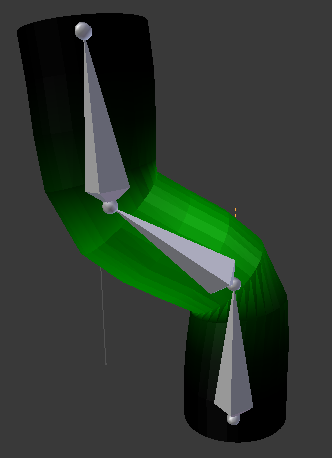
\includegraphics[width=1\linewidth]{wonky_pole/middle_bone}
%         \caption{Middle joint.}
%     \end{subfigure}%
%     \begin{subfigure}{0.25\linewidth}
%     \centering
%         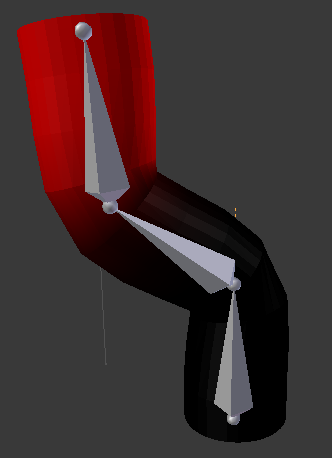
\includegraphics[width=1\linewidth]{wonky_pole/upper_bone}
%         \caption{Upper joint.}
%     \end{subfigure}%
%     \begin{subfigure}{0.25\linewidth}
%     \centering
%         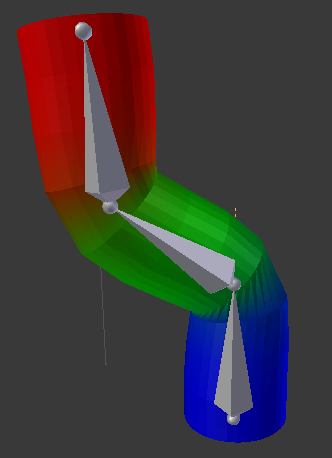
\includegraphics[width=1\linewidth]{wonky_pole/linear_blend}
%         \caption{Linear blend.}
%     \end{subfigure}%
%     \caption{A rigged cylinder with $|J| = 3$ and where each vertex $v_{i} = (x_{i}, s_{i}) \in V$ has a skinning weight vector $s_{i} \in \mathbb{R}^{3}$.}
%     \label{fig:rigged_cylinder}
% \end{figure}

% Figure \ref{fig:rigged_quadruped} shows a more complex rigged quadruped mesh with $|J| = 25$ with skinning weight influences again shown by the linear blend colorization scheme. Again, each joint is assigned a unique RGB value and a vertex's colour is calculated by linearly combining joint colours with skinning weight vectors given by the $\{s_{i}\}$. A triangle's colour is then generated by averaging the colours given for the three surrounding vertices.

% \begin{figure}[H] % Example image
%     \center{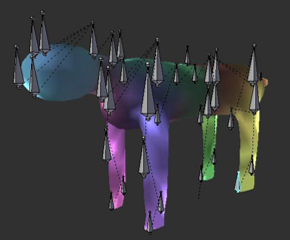
\includegraphics[width=0.5\linewidth]{linear_blend_bold_bones}}
%     \caption{A rigged quadruped with $|J| = 25$ and where each vertex $v_{i} = (x_{i}, s_{i}) \in V$ has a skinning weight vector $s_{i} \in \mathbb{R}^{3}$. Visualization uses the linear blend colorization scheme in which each joint is assigned a unique RGB value.}
%     \label{fig:rigged_quadruped}
% \end{figure}

Once a mesh has been suitably rigged, Linear Blend Skinning (LBS) can be used to apply the mesh deformation. Typically, a user assigns a transformation (e.g. rotation and translation) to each `joint' and LBS computes the an updated position of vertex $v = (x, s)$ where $x$ is the original location and $s = \{s_j\}$ are the skinning weight influence of joints $j$. The matrix $U_{j}$ (occasionally referred to as a the \emph{reference pose}) is the mapping from the bone's "default" coordinate system to world coordinates. As a result, it need only be computed (and inverted) once since it is invariant to changing joint angles. In general, a user will supply the matrices $D_{j}$ to define the mapping from the bone's deformed coordinate system to world coordinates.

The updated position of an input point $x$ can then be calculated by LBS:

\begin{equation}
    LBS(D, x; U, s) = \sum_{j}s_{j}D_{j}U_{j}^{-1}x
\end{equation}

% TODO: Explain LBS for kinematic trees
Note this formulation is made slightly more complicated in the case of kinematic trees, since the 

Similarly to the approach mentioned above, this formulation can again be seen as a generative 3D model. In particular, an output vertex positions $v'$ can be computed from a vector of 3D joint rotations $\theta$ and input vertex position $v$ as follows:

\begin{equation}
    v' = LBS(R(\theta), v)
\end{equation}

\end{definition}

With the above formulation, it is now possible to give an overview of recent hand tracking literature. In many cases, 3D morphable hands models are built to reflect the 27 biological hand bones (occasionally except the capal bones which join the fingers to the wrists). Of course, while the major source of hand deformation is due to 3D pose, some sources of variation are present due to hand size and finger propotions.

Allen et al~\cite{xxx} handle this variation adapting a 3D surface with displacement maps with various constraints designed to avoid self-intersections before adopting the linear blend skinning formulation defined above. Rhee et al~\cite{xxx} learn a shape deformation space (with a similar technique to that of faces) and user-specific skinning weights for LBS. Albrecht undergo a laborious process to create extremely detailed hand models through laser scanninng plaster casts~\cite{xxx}. A significant advance was presented by Taylor et al~\cite{xxx}. who presented a method to learn a personalized hand model (although not a shape basis) given an input video sequence (with depth) taken of a user slowly articulating their fingers. Ballan et al.~\cite{xxx} follow a similar process by making use of multi-view input. 


% TODO: Allen et al. B. Allen, B. Curless, and Z. Popovic. Articulated body de-formation from range scan data. In ACM Transactions on Graphics (TOG). ACM, 2002. 2

% Represent the model as an adaptation of a standard subdivision surface model with linear blend skinning. Cruicially their adaptations are displacement maps on top of a base surface. The displacements must be limited in magnitude to avoid self-intersections and their shape basis is forced to coincide with the input scans.

% % TODO: Rhee et al. T. Rhee, U. Neumann, and J. P. Lewis. Human hand modeling from surface anatomy. In Proceedings of the 2006 symposium on Interactive 3D graphics and games, pages 27–34. ACM, 2006. 2

% Early work included the work of Rhee et al.~\cite{xxx} who learn a 3D shape deformation space from hands by fitting 3D model with user-specific skinning. 

% % TODO: Albrecht et al. I. Albrecht, J. Haber, and H.-P. Seidel. Construction and animation of anatomically based human hand models. In Proc. Eurographics, 2003. 2

% Albrecht et al. go to the other extreme creating very detailed, physically-realistic hand models. However, the process is laborious requiring plaster casting of human hands, performing laser scans, and manually creating a physics-enabled hand model.

% % TODO: Taylor et al. J. Taylor, R. Stebbing, V. Ramakrishna, C. Keskin, J. Shotton, S. Izadi, A. Hertzmann, and A. Fitzgibbon. User-specific hand modeling from monocular depth sequences. In Proc.CVPR, 2014. 1, 2, 4, 5, 7

% A more automatic technique is presented by Taylor et al., which generates personalized hand models given noisy input depth sequences where the user’s hand rotates 180 degrees whilst articulating fingers. A continuous optimization that jointly solves for correspondences and model parameters across a smooth subdivision surface with as rigid as possible (ARAP) regularization leads to high-quality userspecific rigged hand models, though not a shape basis. Whilst the process is automatic, the hands are required to cover the full range of articulations, and longer sequences are required, leading to more complex capture requirements and more costly optimization.

% % TODO: Ballan et al. L. Ballan, A. Taneja, J. Gall, L. V. Gool, and M. Pollefeys. Motion capture of hands in action using discriminative salient points. In Proc. ECCV, 2012. 1, 2

% Ballan et al. construct a personalized hand
% mesh using a multiview camera rig and Poisson surface reconstruction, which is then manually skinned. They demonstrate high-quality results with complex two-handed and
% hand-object interactions, closely fitting the detailed mesh
% model to the data. However, this system focuses on pose
% estimation as opposed to the shape construction, which is
% performed in an time consuming manual manner.

% TODO: Khamis et al. Learning an efficient model of hand shape variation from depth images

% TODO: Fits Like a Glove: Tan et al. https://www.microsoft.com/en-us/research/wp-content/uploads/2016/06/FitsLikeAGlove.pdf



% TODO: Taylor et al. Efficient and Precise Interactive Hand Tracking Through Joint, Continuous Optimization of Pose and Correspondences

\subsection{Modelling the human body surface}

% hasler et al. 2010

However, of all human categories, the works of most relevance to this thesis are those which represent the entire human body surface. It is first important to characterize these two deformation modes which must be overcome with modelling algorithms. Firstly, there is considerable variation in the \emph{shape} characteristics between different human subjects. Humans not only vary in their heights and weights, but also in their body part proportions, muscle density, fat etc. Secondly, humans exhibit significant \emph{pose} variation, characterized by the range of motion of body parts (e.g. arms and legs). In general, pose is likely to change for a individual subject over a sequence. 

The earliest deformable 3D models of the human body was presented by Allen at al~\cite{xxx} (although ~\cite{xxx} came soon after with similar ideas). Allen et al. learnt a PCA shape space model from 250 registered body scans cound in the CAESAR dataset. The model was articulated through a set of pose parameters, which use linear blend skinning to interpolate rotation matrices assigned to the joint to transform model veertices. Unfortunately, this approach suffers from artefacts around joint locations, due to a loss of volume. For this reason, it is important to note that pose and shape are not entirely independent; in fact, body shape does indeed change due to pose variation. Imagine for example, how a fatty stomach region would deform during a walking sequence. SCAPE~\cite{anguelov05scape} improved over this by introducing a model equipped with both body shape variation and pose-dependent shape changes, expressed in terms of triangle deformations (rather than vertex displacements, see~\cite{loper15smpl} for a comprehensive overview). An important advance was made by Hasler et al.~\cite{xxx}, who learn two linear blend rigs: one for pose and one for body shape. In this model, shape change was controlled through the introduction of abstract bones that further deform the vertices.

Perhaps the most significant advance however, was the introduction of the Skinned Multi-Person Linear (SMPL) model of Loper et al.~\cite{loper15smpl}. SMPL follows a similar design philosophy to SCAPE by decomposing shape into identity-dependent and pose-dependent components. However, unlike scape, SMPL adopts a vertex-based skinning approach based on corrective blend shapes. The model's shape space is first taught how human beings deform through pose changes using 1786 high-resolution 3D scans of different subjects in a wide variety of poses. Following alignment to a template mesh, a linear model for each biological gender is created from the CAESAR dataset \cite{robinette2002civilian} using principal component analysis (PCA). SMPL can then be viewed as a function, which makes use of a shape basis and linear blend skinning to map a set of pose and shape parameters to a set of vertex locations. Precisely, \emph{pose} is given as a set of 3D rotations (per-joint and global) in axis-angle form $\pose \in \R{24}{3}$. \emph{Shape} is then given as coefficients for a learned shape basis $\shape \in \R{10}$. The SMPL function can then be viewed as:

\begin{equation}
    v = \SMPL(\pose, \shape) + \trans
\end{equation}

where $v \in \RR{6890}{3}$ and $\trans \in \R{3}$ is a global translation parameter. Further details on SMPL have been left to Chapter 5 of this thesis, which makes use of the model to examine uncertainty when deriving 3D reconstructions of ambiguous input imagery.

% Another key ambition for the SMPL model was the motivatio to create a realistic data-driven human body model which can be rendered in real-time using standard engines, such as Unity~\cite{unity2017} or Blender~\cite{blender2017}. Having been designed for animation, SMPLs base template has a number of useful qualities for this work; the underlying mesh is a clean structure and comprises relatively few polygons. A novelty of this model is that it encodes explicit and meaningful body joint positions. Some sample SMPL meshes are shown in Figure \ref{fig:smpl_model}.

% TODO: GHUML & GHUM model
More recently, SMPL has been combined with face and hand models to add expressive capabilities~\cite{xiang19monocular, joo18total, pavlakos19expressive}. CAPE~\cite{CAPE:CVPR:20} also shows how to add a clothing parameter to effectively model humans in clothing, a challenge solved by learning a shape prior over freeform vertex deformations Techniques have also been developed to model human clothing -- a common challenge generally handled by allowing SMPL model vertices to vary independently to the provided blend shapes. SMPL has also been recently improved with STAR~\cite{STAR:2020} which constructs a part-based shape space (closely related to the local PCA space discussed in the earlier shape section of this literature review). They show this new parameterization is much more efficient (uses approximately 20\% of the model parameters of SMPL) and avoids capturing spurious long-range correlations present in the training dataset. They also show a method for learning shape-dependent pose-corrective blendshapes, that better model how individuals with different body shapes deform with motion. Tangential work of Xu et al.~\cite{ghum-ghuml} train an end-to-end network and learn 3D human body model parameters (including faces and hands) for an input artist model using variational auto-encoders and normalizing flows. This work will be further explored Chapter 5 in which these generative models will be fully examined. 

\begin{figure}[H] % Example image
    \center{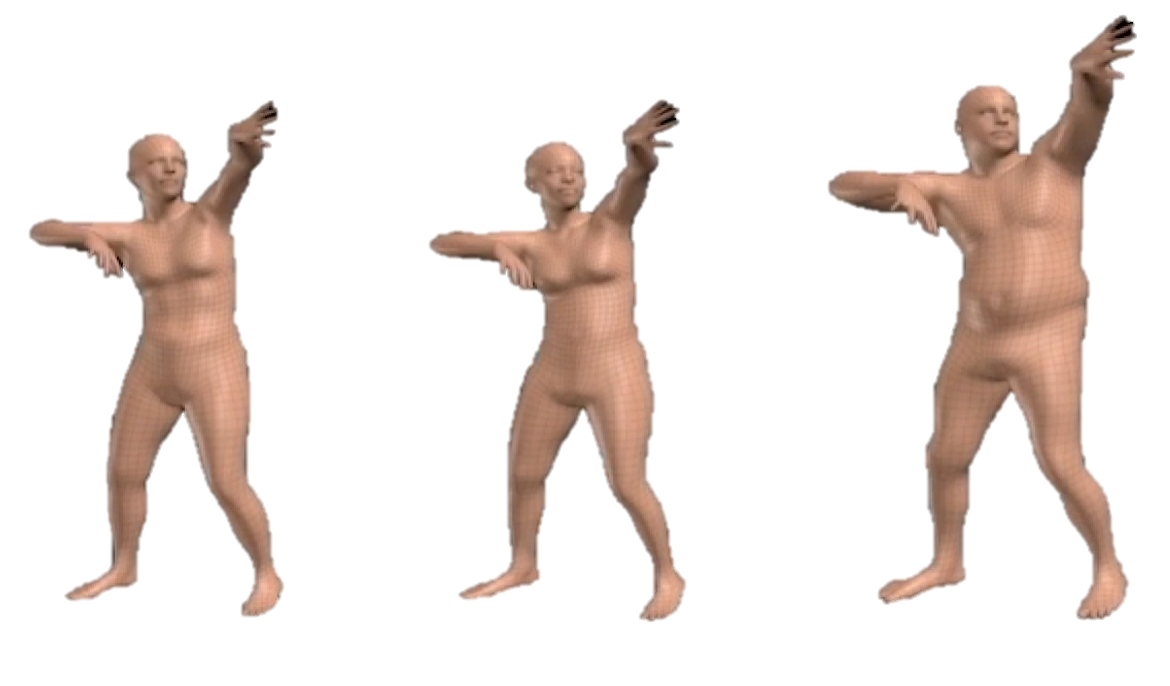
\includegraphics[width=0.5\linewidth]{smpl_wbg}}
    \caption{SMPL model showing pose-invariant shape changes, reprinted from~\cite{loper15smpl}.}
    \label{fig:smpl_model}
\end{figure}

\subsection{Modelling animals}

There is still relevatively little work specifically focusing on the 3D scanning~\cite{xxx} and modelling of animal categories. The variation in animal shape and sizes combined with the practical challenges associated with scanning live animal subjects (particularly in attaching traditional motion capture equipment) make scanning a difficult task. As a result, there is a significant lack of real 3D animal training data available in the public domain which could otherwise have been employed to build 3D deformable models. As with humans, animals deformations can again be factored into shape (e.g. variation mostly due to identity) and pose (variation due to articulated motion). However, the enormous diversity among animal species and even between individual breeds results in a much more complex shape space.

Some early work by Favreau et al~\cite{xxx} describe a method for animating an artist-designed rigged 3D model, by tracking a 2D sequence. Chen et al.~\cite{xxx} learn a shape space by registering 11 3D shark models downloaded from the Internet. Cashman et al.~\cite{xxx} learn a morphable model of dolphin shapes by adapting a representative 3D model to 2D images. Ntouskos et al.~\cite{xxx} fit geometric primitives to manually-segemented animal parts generated from an input collection. Reinert et al.~\cite{xxx} demonstrates an effective method for fitting generalized cylinders to an input video sequence supplied with sketched limb tracks. They demonstrate reconstructed results with 3D texture on a few quadruped sequences. So far, none of these techniques for animal reconstruction explicitly factor shape and pose.

\subsubsection{SMAL}
A similar technique to that used to build the SMPL model has been recently used to build a Skinned Multi-Animal Linear Model (SMAL)~\cite{zuffi2017menagerie}, a generative animal model exhibiting realistic 3D shape (see Figure \ref{fig:smal_model_shape}) and pose (see Figure \ref{fig:smal_model_poses}). Due to the lack of available motion capture data for animal subjects, the SMAL model is learnt from a set of $41$ 3D scans of toy figurines in arbitrary poses. The figurines span five quadruped families, and included examples of lions, cats, tigers, dogs, horses, any many more, although notably for this work no rodent toys were included. The paper introduces a new technique to accurately align each toy scan to a common template, allowing the shape space to be learnt.

\begin{figure}[H]
    \centering
    \begin{subfigure}{0.3\linewidth}
    \centering
        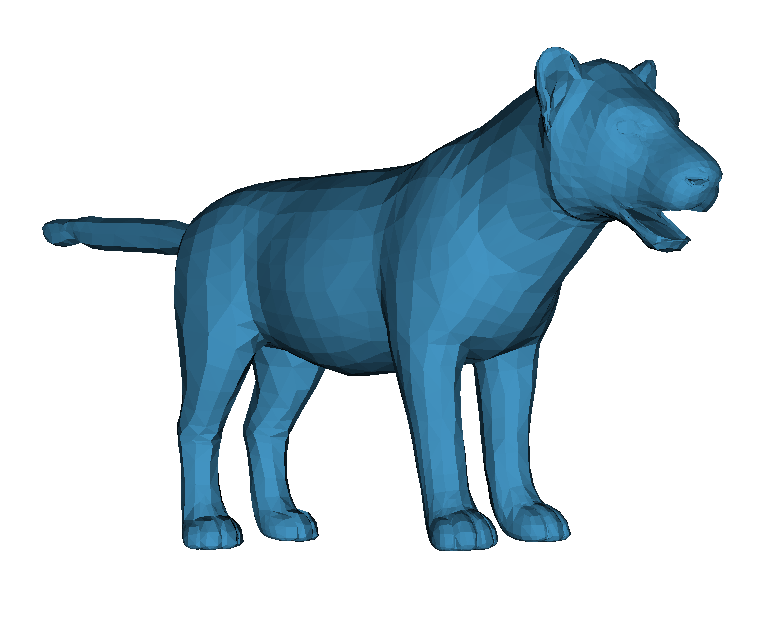
\includegraphics[width=1\linewidth]{smal/default}
        \caption{Default SMAL mesh.}
    \end{subfigure}%
    \begin{subfigure}{0.3\linewidth}
    \centering
        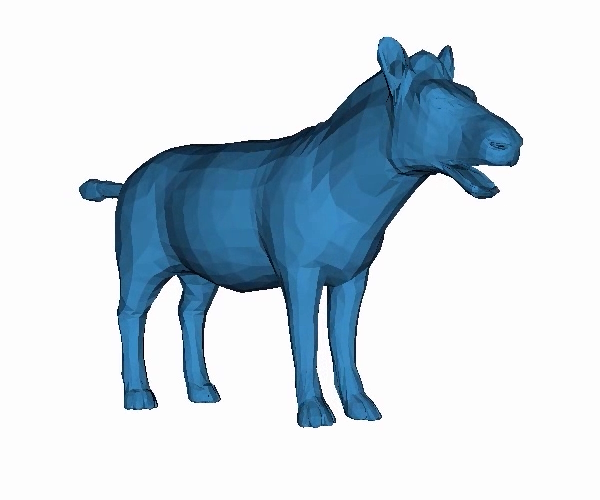
\includegraphics[width=1\linewidth]{smal/horse}
        \caption{SMAL in horse shape.}
    \end{subfigure}%
    \begin{subfigure}{0.3\linewidth}
        \centering
            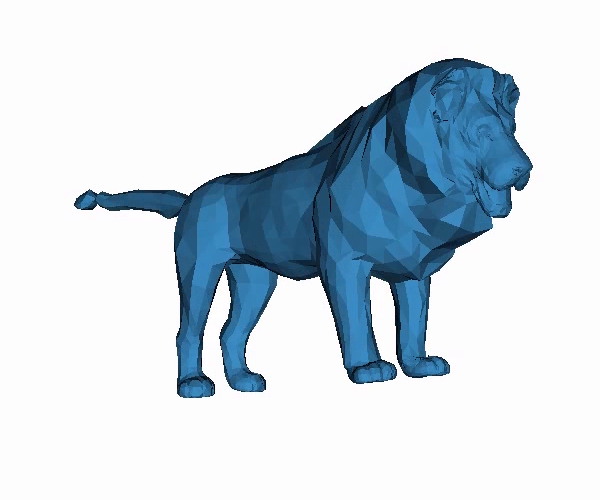
\includegraphics[width=1\linewidth]{smal/lion}
            \caption{SMAL in lion shape.}
    \end{subfigure}%
    \caption{SMAL with varying shape parameters.}
    \label{fig:smal_model_shape}
    \end{figure}

    \begin{figure}[H]
    \centering
    \begin{subfigure}{0.3\linewidth}
    \centering
        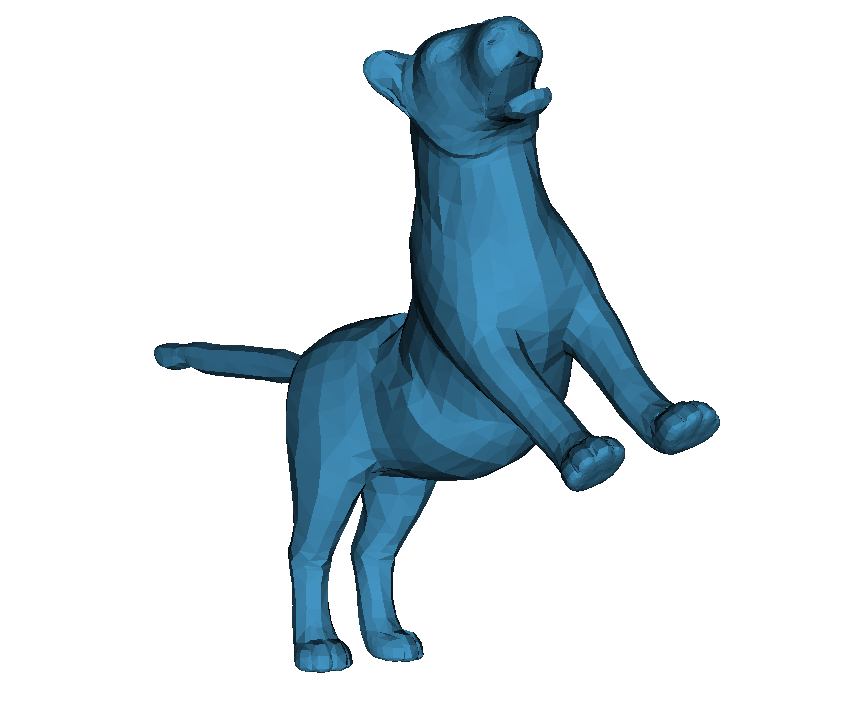
\includegraphics[width=1\linewidth]{smal/pose_1}
    \end{subfigure}%
    \begin{subfigure}{0.3\linewidth}
    \centering
        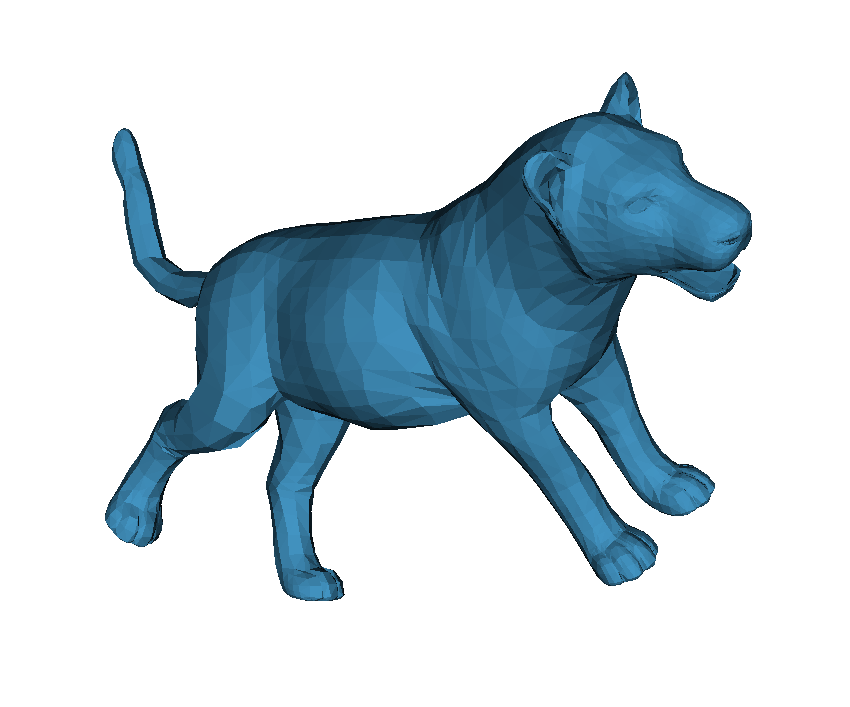
\includegraphics[width=1\linewidth]{smal/pose_2}
    \end{subfigure}%
    \begin{subfigure}{0.3\linewidth}
        \centering
            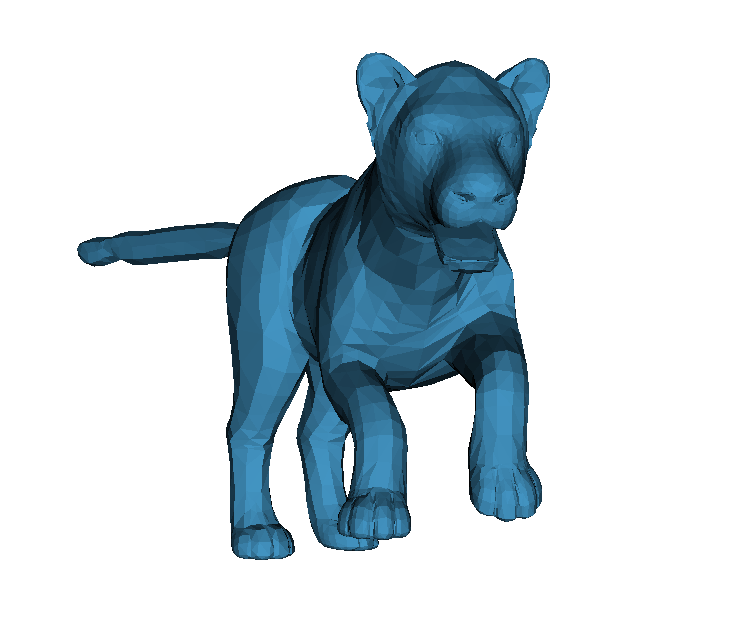
\includegraphics[width=1\linewidth]{smal/pose_3}
    \end{subfigure}%
    \caption{SMAL with varying pose parameters.}
    \label{fig:smal_model_poses}
\end{figure}

From the paper, SMAL is defined as a function $\SMAL(\pose, \shape)$ parameterized by pose-invariant shape $\shape \in \R{41}$ (again, coefficients of a low-dimensional shape space) and pose $\pose \in \RR{32}{3}$ (including global rotation). There are three pose parameters for each of the $32$ body joints and an additional three to express the global rotation. Global translation $\gamma$ is expressed by a further three parameters. The $\SMAL$ function returns a triangulated surface comprising $6890 \times 3$ vertex locations. Chapters 3 and 4 of this thesis make use of the SMAL model in order to reconstruct various quadruped categories.
